\subsubsection{Key Extraction}
\label{sec:sphinx:keyderivation}

Path selection, see section \ref{sec:path-selection}, results in a list $n_0, \dots, n_r$ of mixnodes which are supposed to process and forward the packet before the message reaches its destination $dest$. HOPR nodes use their public keys as addresses, hence the public keys $Y_0, \dots , Y_r$ are known to the creator of a packet.

\paragraph{Key Exchange}

Having this knowledge allows the creator of the packet to perform an offline Diffie-Hellman key exchange with each of the mix nodes $n_0 , \dots , n_r$ and the destination $dest$, resulting in shared secrets $s_0, \dots , s_r$ and $s_{dest}$.

To provide perfect forward secrecy and thereby minimize the risk of key corruption, the sender first samples a random value $x \in \mathbb{F}$ and derives $\alpha_0 = x \cdot G$. It further derives blinding factor $b_0$ as $b_0 = \mathsf{KDF}(\alpha_0, x \cdot Y_0)$ where $\mathsf{KDF}(salt, secret)$ is a key derivation function, see appendix \ref{appendix:keyderivation}, and derives the shared secret as $s_0 = x \cdot b_0 \cdot Y_0$. Hence, deriving the shared secret $s_0$ requires the knowledge of the sender's field element $\alpha_0 = x \cdot G$ as well as the receivers' field element $x \cdot b_0 \cdot Y_0$.

The first relayer $n_0$ is then able to compute $s_0$ by first deriving $x \cdot Y_0$ as

$$y_0 \cdot \alpha_0 = y_0 \cdot x \cdot G = x \cdot ( y_0 \cdot G) = x \cdot Y_0$$

yielding $b_0$ and $s_0 = y_0 \cdot b_0 \cdot \alpha_0$ where $y_0$ refers to the private key of node $n_0$. The value $s_0$ then servers as a master secret to perform further key derivations as described in appendix \ref{appendix:keyderivation}.

\paragraph{Transformation}

Once the key extraction is done, the each relayer $n_i$ transforms its value $\alpha_i$ into $\alpha_{i+1}$ by setting $\alpha_{i+1} = b_i \cdot \alpha_i$ such that

$$ \alpha_i = x \cdot \biggl(\prod_{j=0}^{i} b_j \biggr) \cdot G = \biggl(\prod_{j=0}^{i} b_j \biggr) \cdot \alpha_0 = \biggl(\prod_{j=k+1}^{i} b_j \biggr) \cdot \alpha_k $$

By adding an additional blinding for every node along the selected path, each incoming $\alpha_i$ and each outgoing $\alpha_{i+1}$ become indistinguishable from random numbers of the same length. Hence, an adversary who observes incoming and outgoing packets cannot use $\alpha$ to track packets.

Since each $s_{i+1}$ depends on $b_{i+1}$ and therefore on all $\alpha_0, \dots , \alpha_i$, the key extraction can only be done in the foreseen order; first derive $s_0$, then derive $s_1$ etc. Hence, an adversary is unable to extract keys in a more favorable order, e.g. because it has managed to compromise \textit{some} but not \textit{all} nodes on the path.

\paragraph{Example}

The following example shows the key extraction process for a sender $A$, three mix nodes $B,C,D$ and a receiver $Z$.

\begin{align*}
    (\alpha_B,b_B,s_B) & = (x \cdot G,\textsf{KDF}(\alpha_B, y_B \cdot \alpha_B), y_B \cdot \alpha_B )                   \\
    (\alpha_C,b_C,s_C) & = (x \cdot b_B \cdot G,\textsf{KDF}(\alpha_C, y_C \cdot \alpha_C), y_C \cdot \alpha_C )             \\
    (\alpha_D,b_D,s_D) & = (x \cdot b_B \ b_C \cdot G,\textsf{KDF}(\alpha_D, y_D \cdot \alpha_D), y_D \cdot \alpha_D )       \\
    (\alpha_Z,b_Z,s_Z) & = (x \cdot b_B \ b_C \ b_D \cdot G,\textsf{KDF}(\alpha_Z, y_Z \cdot \alpha_Z), y_Z \cdot \alpha_Z ) \\
\end{align*}

where $y_i$ for $i \in \{ B,C,D,Z \}$ refers to the nodes' private keys and $s_i$ denotes the derived shared secret group elements.

Packets consist of $(\alpha, \beta, \gamma)$ where $\beta$ is described in section \ref{sec:sphinx:routinginformation} and $\gamma$ in section \ref{sec:sphinx:integrity}, leaving both underspecified for the moment. Let further be $packet_i = (\alpha_i, \beta_i, \gamma_i)$, leading to:

\begin{figure}[H]
    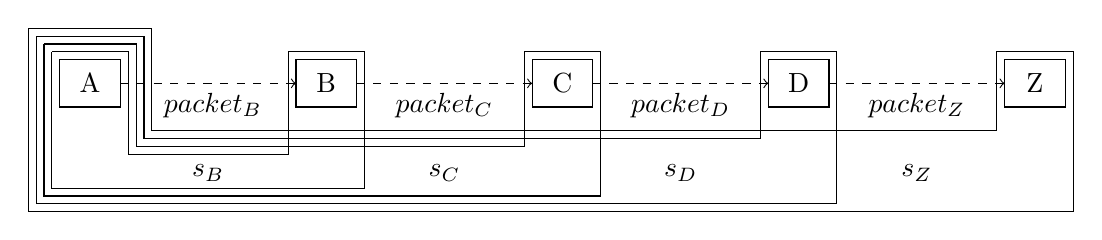
\begin{tikzpicture}
        \def\offset{3}
        \def\nodeWidth{0.77}
        \def\padding{0.93}
        \def\lowerpadding{0.7}
        \def\nodeHeight{0.6}
        \foreach \i\name\bi\packetName in{0/A/0/$packet_A$,1/B/$b_B$/$\ packet_B$,2/C/${b_C}$/$packet_C$,3/D/$b_D$/$packet_D$,4/Z/$b_Z$/$packet_Z$} {
                \draw (\i*\offset,0) rectangle (\i*\offset+\nodeWidth,\nodeHeight) node [midway] {\name};

                \ifnum\i>0
                    \draw (-0.1*\i,\nodeHeight+0.1*\i) -- (-0.1*\i,-\padding-0.1*\i) -- (\i*\offset+0.1+\nodeWidth,-\padding-0.1*\i) -- (\i*\offset+0.1+\nodeWidth,\nodeHeight+0.1) -- (\i*\offset-0.1,\nodeHeight+0.1) -- (\i*\offset-0.1,-\lowerpadding+0.1*\i) -- (\nodeWidth+0.1*\i,-\lowerpadding+0.1*\i) -- (\nodeWidth+0.1*\i,\nodeHeight+0.1*\i) -- (-0.1*\i,\nodeHeight+0.1*\i);
                \fi

                \ifnum\i>0
                    \draw [->,dashed] (\i*\offset-\offset+\nodeWidth,0.3) -- (\i*\offset,0.3) node [midway,below] {\packetName} node [midway,below=26pt] {{\smaller$s_{\name}$}};
                \fi
            }
    \end{tikzpicture}
    \caption{Node $A$ derives shared keys $s_B,s_C,s_D,s_Z$ with node $B,C,D,Z$ using their public keys $Y_B,Y_C,Y_D,Y_Z$.}
    \label{fig:sphinx:keyderivation}
\end{figure}
